\documentclass[aspectratio=54]{beamer}

%
% Choose how your presentation looks.
%
% For more themes, color themes and font themes, see:
% http://deic.uab.es/~iblanes/beamer_gallery/index_by_theme.html
%
\mode<presentation>
{

	\usetheme{PaloAlto}	
	\usecolortheme{default}
	\usefonttheme[onlymath]{serif}	
 
 \setbeamercolor{normal text}{fg=black}
\setbeamercolor{alerted text}{fg=black}
\setbeamercolor{author}{fg=blue}
\setbeamercolor{institute}{fg=blue}
\setbeamercolor{date}{fg=green}
\setbeamercolor{frametitle}{fg=white}
\setbeamercolor{framesubtitle}{fg=brown}
\setbeamercolor{block title}{bg=blue, fg=white}		%Cor do título
\setbeamercolor{block body}{bg=gray, fg=darkgray}	%Cor do texto (bg= fundo; fg=texto)
%  \setbeamertemplate{navigation symbols}{}
%  \setbeamertemplate{caption}[numbered]
}

\usepackage{textpos} 
\usepackage{etoolbox}
\usepackage{fancybox}
\usepackage[comma,numbers,sort&compress]{natbib}
\usepackage{hyperref}
\usepackage[brazil]{babel}
\usepackage[utf8x]{inputenc}


\hypersetup{
    colorlinks=true,
    citecolor=green,
    linkcolor=red,
    backref=true
}
\everymath{\color{blue}}
\let\oldbibitem=\bibitem
\renewcommand{\bibitem}[2][]{\label{#2}\oldbibitem[#1]{#2}}
\let\oldcite=\cite
\renewcommand\cite[1]{\hypersetup{linkcolor=gray} \hyperlink{#1}{\oldcite{#1}}}
\let\oldcitep=\citep
\renewcommand\citep[1]{\hypersetup{linkcolor=gray}\hyperlink{#1}{\oldcitep{#1}}}
%\let\oldciteauthor=\citeauthor
%\renewcommand\citeauthor[1]{\hypersetup{linkcolor=green}\hyperlink{#1}{\oldciteauthor{#1}}} 
%
\let\oldcitet=\citet
\renewcommand\citet[1]{\hypersetup{linkcolor=gray}\hyperlink{#1}{\oldcitet{#1}}} 

\logo{
\includegraphics[width=1.6cm,height=1.4cm]{img/uem2.pdf}}
% --- Informações do documento ---

\title{Experimento x\\
\small }

 
\author[]{
Tiririca\\%
Einsten da silva \\
José Cristo\\
Compadre Washington  \\%- RA:PG47547}
}
\institute{
Prof.\textordfeminine Edson \\
Mestrado em Ciência da Computação \\
Departamento de Informática}
\date{\today, v-0.3} 

\makeatletter
\setlength{\beamer@headheight}{1.4cm}
  \setbeamertemplate{sidebar \beamer@sidebarside}%{sidebar theme}
  {
  
    \beamer@tempdim=\beamer@sidebarwidth%
    \advance\beamer@tempdim by -6pt%
    \insertverticalnavigation{\beamer@sidebarwidth}%
    \vfill
    \ifx\beamer@sidebarside\beamer@lefttext%
    \else%
      \usebeamercolor{normal text}%
      \llap{\usebeamertemplate***{navigation symbols}\hskip0.1cm}%
      \vskip2pt%
    \fi%
}%
\newcommand{\argmax}[1]{\underset{#1}{\arg\max}\;}
\makeatother
\begin{document}

\begin{frame} 
	\frametitle{ \fontsize{20pt}{11pt} \selectfont Universidade Estadual de Maringá}
									 
									
	\titlepage
									
\end{frame}
\begin{frame}{Tópicos}
	\tableofcontents[sections={1-10}] 
\end{frame}
%\begin{frame}{Sumário}
%   \tableofcontents[sections={7-}] 
%\end{frame}
 

% Uncomment these lines for an automatically generated outline.
%\begin{frame}{Outline}
%  \tableofcontents
%\end{frame}


\section{Introdução}



\begin{frame}{Introducao\cite{Vieira2006}}
	
	\begin{itemize}
	\item blabla
	\pause
	\item As LLC sao tipo 2 da hierarquia de Chomsky.
	\pause
	\item Bombeamento para LLC.
	\end{itemize} 
	 
\end{frame}


\input{txt/part2}
\input{txt/part3}
\input{txt/part4}



\section{Finalização}
\subsection{Perguntas}
\begin{frame}{Perguntas}
	\begin{figure}
		\centering
		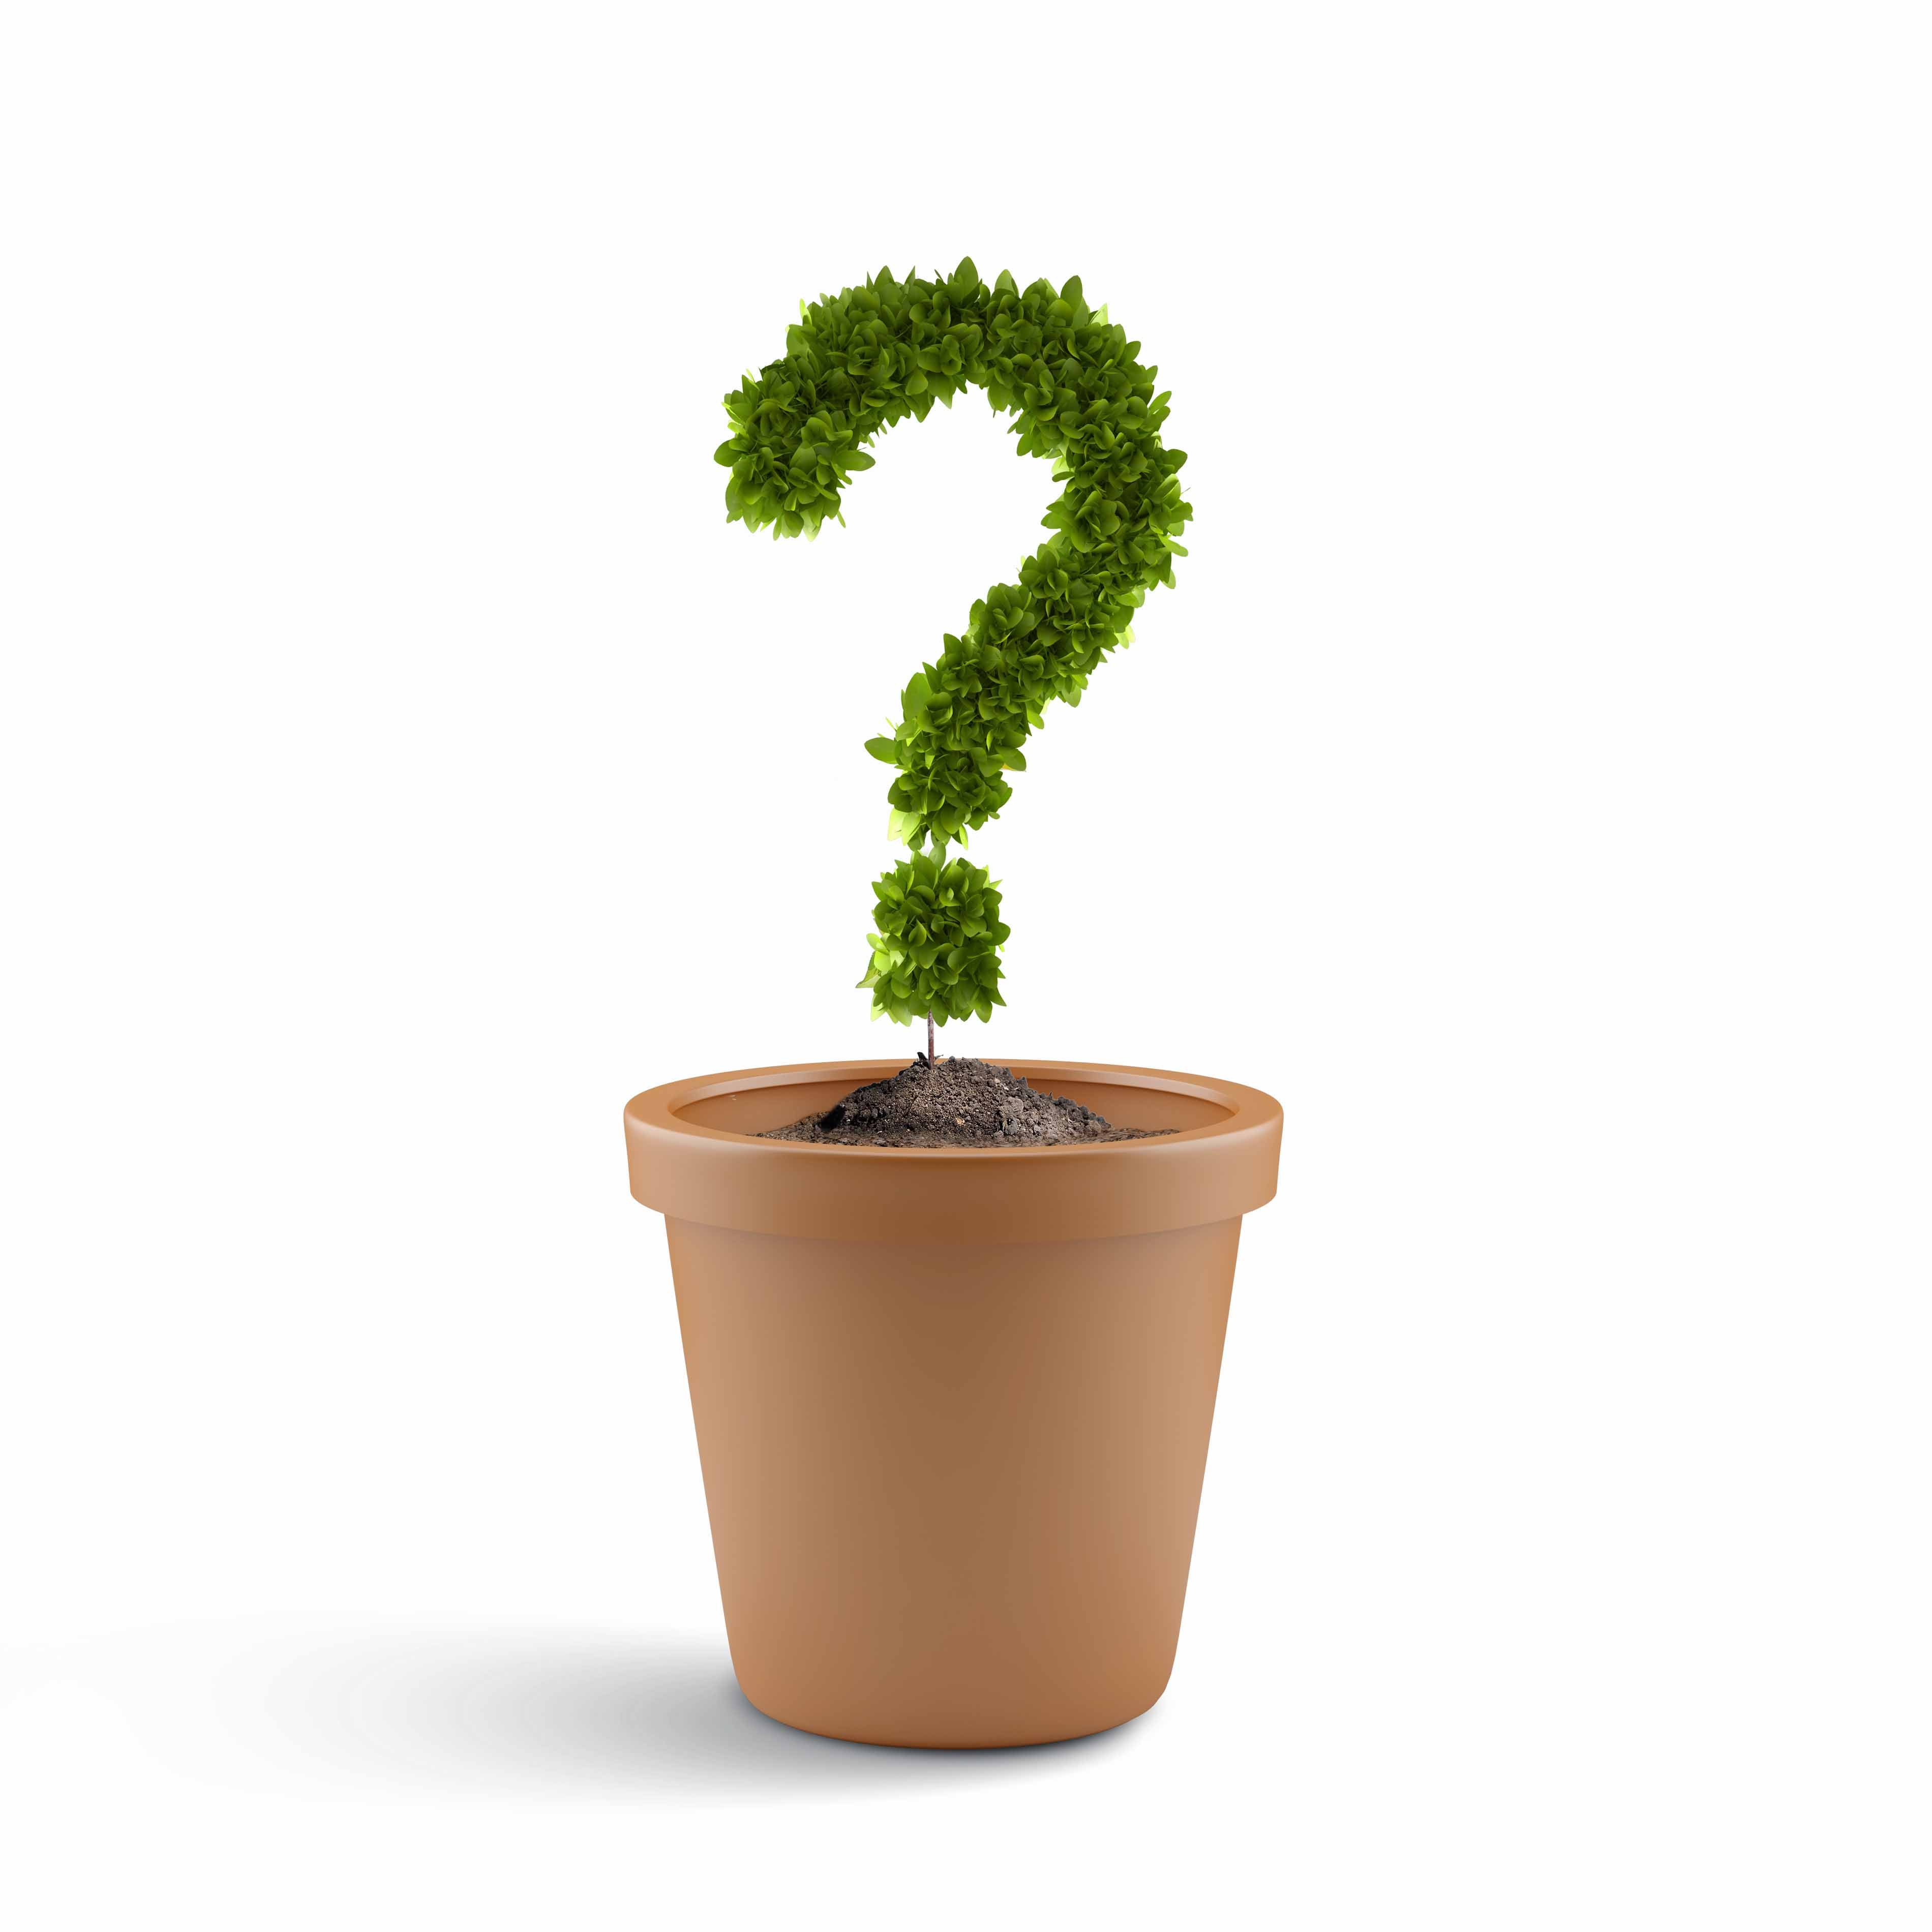
\includegraphics[width=7cm,keepaspectratio=true]{img/ask.jpg}
	\end{figure}
\end{frame}

\subsection{Agradecimento}
\begin{frame}{Agradecimento}
	\begin{figure}
		\centering
		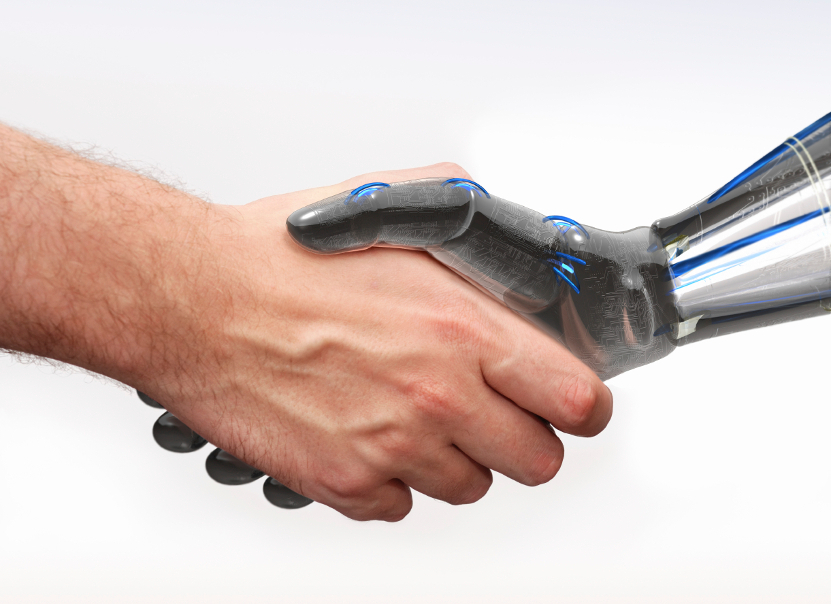
\includegraphics[width=7cm,keepaspectratio=true]{img/hand.jpg}
	\end{figure}
\end{frame}


\begin{frame}[allowframebreaks]{Referências}
	\bibliographystyle{abbrvnat}
	\bibliography{referencias}
\end{frame}

\end{document}
